\subsection{How to setup a version-controlled EAP file}

The following assumes an EAP file has already been placed under version control as instructed in the previous section, and that you wish to checkout this file
and work with it. If our instructions do not work, the EAP file may have been placed under version control in a different manner. If this is the case, please
contact whoever checked in the file, and setup the file for working with EA and SVN for further instructions.

\begin{enumerate}

\item[$\blacktriangleright$] Check-out the project with the EAP file from the server using Tortoise-SVN or Eclipse/Subclipse (or any SVN client of your
choice). You should now have a \textit{.svn} folder in the directory where you saved the revision.

\item[$\blacktriangleright$] Open the EAP file. If the EAP file is already under version control \emph{and} has been set-up correctly, a dialogue similar to
\Cref{fig:advanced-topics-eaSVN-incompleteConf} should immediately pop-up.

\item[$\blacktriangleright$] Click ``Yes" to open the ``Version Control Settings'' dialogue (\Cref{fig:advanced-topics-eaSVN-setWorkingCopyPath}).

\begin{figure}[!htbp]
\begin{center}
	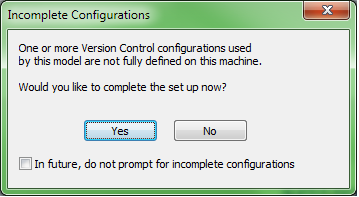
\includegraphics[width=0.6\textwidth]{011}
	\caption{Configure an EAP file which is already under version control}
  	\label{fig:advanced-topics-eaSVN-incompleteConf}
\end{center}
\end{figure}

   \item[$\blacktriangleright$] To work with the EAP file, you now have to \emph{redefine} the SVN variable for the file in your EA workspace.
   To accomplish this, choose the local path to the folder which contains the EAP file in the ``Working Copy Path'' text-box, and correct the value in
   ``Subversion Exe Path'' if necessary (to fit your Slik installation location).

\begin{figure}[!htbp]
\begin{center}
	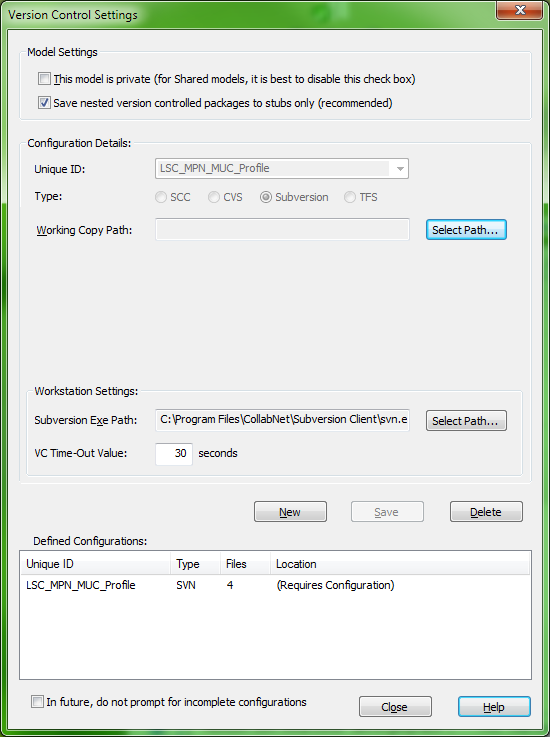
\includegraphics[width=0.9\textwidth]{012}
	\caption{Update settings as required}
  	\label{fig:advanced-topics-eaSVN-setWorkingCopyPath}
\end{center}
\end{figure}

\end{enumerate}
